\section{\texttt{rgl}}

\subsection{Descrição}

% ----------------------------------------------------------------------

\begin{frame}

  \texttt{rgl} é uma biblioteca de funções para visualização interativa
  de gráficos em 3D.  \vspace{2em}
  
  \begin{itemize}
  \item Autores: Daniel Adler, Duncan Murdoch, e outros.
  \item Lançamento: 04-Mar-2004.
  \item Versão: 0.95.1247.
  \item URL:
    \url{http://cran.r-project.org/web/packages/rgl/index.html}.
  \end{itemize}

\end{frame}

% ----------------------------------------------------------------------

\begin{frame}
 
  \begin{itemize}
  \item Funções inspiradas nas 2D, de primitivas à médio e alto nível.
    \newline \vspace{-2em}
\setlength{\columnsep}{5pt}
\begin{multicols}{2}
\begin{knitrout}\footnotesize
\definecolor{shadecolor}{rgb}{0.969, 0.969, 0.969}\color{fgcolor}\begin{kframe}
\begin{alltt}
\hlkwd{require}\hlstd{(graphics)}

\hlkwd{plot}\hlstd{(...)}
\hlkwd{persp}\hlstd{(...)}
\hlkwd{points}\hlstd{(...)}
\hlkwd{lines}\hlstd{(...)}
\hlkwd{abline}\hlstd{(...)}
\hlkwd{segments}\hlstd{(...)}
\hlkwd{text}\hlstd{(...)}
\hlkwd{mtext}\hlstd{(...)}
\hlkwd{legend}\hlstd{(...)}
\hlstd{...}
\end{alltt}
\end{kframe}
\end{knitrout}

\begin{knitrout}\footnotesize
\definecolor{shadecolor}{rgb}{0.969, 0.969, 0.969}\color{fgcolor}\begin{kframe}
\begin{alltt}
\hlkwd{require}\hlstd{(rgl)}

\hlkwd{plot3d}\hlstd{(...)}
\hlkwd{persp3d}\hlstd{(...)}
\hlkwd{points3d}\hlstd{(...)}
\hlkwd{lines3d}\hlstd{(...)}
\hlkwd{abclines3d}\hlstd{(...)}
\hlkwd{segments3d}\hlstd{(...)}
\hlkwd{text3d}\hlstd{(...)}
\hlkwd{mtext3d}\hlstd{(...)}
\hlkwd{legend3d}\hlstd{(...)}
\hlstd{...}
\end{alltt}
\end{kframe}
\end{knitrout}
\end{multicols}

%\pause
%\vspace{-0.6cm}
%\begin{knitrout}\footnotesize
%\definecolor{shadecolor}{rgb}{0.969, 0.969, 0.969}\color{fgcolor}\begin{kframe}
%\begin{alltt}
%\hlkwd{snapshot3d}\hlstd{(}\hlkwc{filename}\hlstd{=}\hlstr{"fig3d"}\hlstd{)}
%
%\hlkwd{rgl.postscript}\hlstd{(}\hlstr{"fig3d.pdf"}\hlstd{,}
%               \hlstr{"pdf"}\hlstd{,}
%               \hlkwc{drawText}\hlstd{=}\hlnum{FALSE}\hlstd{)}
%
%\hlkwd{writeWebGL}\hlstd{(...)}
%\end{alltt}
%\end{kframe}
%\end{knitrout}

  \item Representações em 3D de gráficos e de objetos geométricos
    (cubos, elipses, etc).
  \item A visualização em tela com OpenGL, em HTML com WebGL.
  \item Controle com arrastos e cliques de mouse.
  \end{itemize}
  \vspace{2em}

\end{frame}

\frame{
  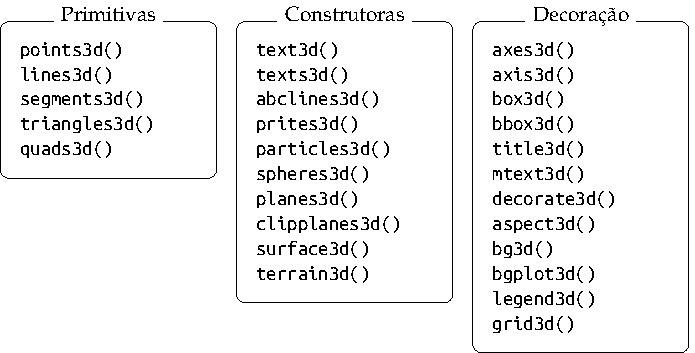
\includegraphics{./tikz/rgl-2.pdf}
}

\subsection{Como usar}

\begin{frame}
  \begin{columns}
    \column{0.70\textwidth} \begin{knitrout}
\definecolor{shadecolor}{rgb}{0.969, 0.969, 0.969}\color{fgcolor}\begin{kframe}
\begin{alltt}
\hlkwd{require}\hlstd{(rgl)}

\hlcom{## Diagrama de dispersão.}
\hlkwd{with}\hlstd{(rock,} \hlkwd{plot}\hlstd{(}\hlkwc{x}\hlstd{=area,} \hlkwc{y}\hlstd{=peri))}           \hlcom{## graphics}
\hlkwd{with}\hlstd{(rock,} \hlkwd{plot3d}\hlstd{(}\hlkwc{x}\hlstd{=area,} \hlkwc{y}\hlstd{=peri,} \hlkwc{z}\hlstd{=perm))} \hlcom{## rgl}

\hlstd{fun} \hlkwb{<-} \hlkwa{function}\hlstd{(}\hlkwc{x}\hlstd{,} \hlkwc{y}\hlstd{)\{}
    \hlkwd{sin}\hlstd{(}\hlkwd{sqrt}\hlstd{(x}\hlopt{^}\hlnum{2}\hlopt{+}\hlstd{y}\hlopt{^}\hlnum{2}\hlstd{))}\hlopt{/}\hlkwd{sqrt}\hlstd{(x}\hlopt{^}\hlnum{2}\hlopt{+}\hlstd{y}\hlopt{^}\hlnum{2}\hlstd{)}
\hlstd{\}}

\hlstd{x} \hlkwb{<-} \hlstd{y} \hlkwb{<-} \hlkwd{seq}\hlstd{(}\hlopt{-}\hlnum{8}\hlstd{,} \hlnum{8}\hlstd{,} \hlkwc{by}\hlstd{=}\hlnum{0.25}\hlstd{)}
\hlstd{z} \hlkwb{<-} \hlkwd{outer}\hlstd{(x, y, fun)}

\hlcom{## Superfície.}
\hlkwd{persp}\hlstd{(}\hlkwc{x}\hlstd{=x,} \hlkwc{y}\hlstd{=y,} \hlkwc{z}\hlstd{=z)}   \hlcom{## graphics}
\hlkwd{persp3d}\hlstd{(}\hlkwc{x}\hlstd{=x,} \hlkwc{y}\hlstd{=y,} \hlkwc{z}\hlstd{=z)} \hlcom{## rgl}

\hlcom{## Não fechar a janela do openGL.}
\hlkwd{snapshot3d}\hlstd{(}\hlstr{"fig3d-1.png"}\hlstd{)}
\hlkwd{rgl.postscript}\hlstd{(}\hlkwc{filename}\hlstd{=}\hlstr{"fig3d.pdf"}\hlstd{,} \hlkwc{fmt}\hlstd{=}\hlstr{"pdf"}\hlstd{)}
\hlkwd{writeWebGL}\hlstd{()} \hlcom{## exporta para webGL.}
\end{alltt}
\end{kframe}
\end{knitrout}

    \column{0.29\textwidth}
    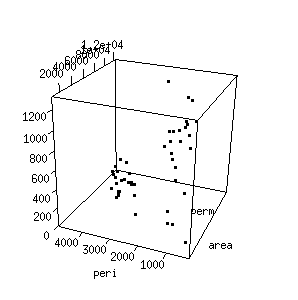
\includegraphics[width=\linewidth]{./images/fig3d-1.png}\\
    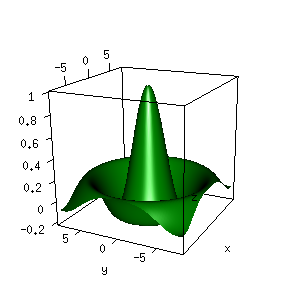
\includegraphics[width=\linewidth]{./images/fig3d-2.png}
  \end{columns}
\end{frame}

% ----------------------------------------------------------------------

\subsection{Exemplos}

\begin{frame}

  Praticando:
  \begin{enumerate}
  \item \href{run:../rgl/rgl.html}{Galeria rgl iguir2}
  \end{enumerate}

  \vspace{0.5cm} Algumas aplicações com o rgl:
  \begin{itemize}
  \item
    \href{http://cran.r-project.org/web/packages/rgl/vignettes/}{Galeria
      do autor}
  \item \href{http://www.r-bloggers.com/?s=rgl}{Busca no R Bloggers}
  \end{itemize}

\end{frame}
